\documentclass[11pt,a4paper]{article}
\usepackage{times,latexsym}
\usepackage{url}
\usepackage[T1]{fontenc}
\usepackage[]{tacl2021v1}  % submission: anonymous, line numbers, confidential header; [acceptedWithA] for the final version
\usepackage{amsmath,amssymb}
\usepackage{booktabs,tabularx,array}
\usepackage{tikz}
\usetikzlibrary{arrows.meta,positioning,fit,backgrounds,calc,shapes.geometric,shapes.misc}
\graphicspath{{../../figures/}}
\tikzset{>={Stealth[length=1.8mm]},
  box/.style={draw, rounded corners=2pt, align=center, font=\scriptsize, minimum height=7mm, inner sep=2pt, fill=#1}, box/.default=cyan!8,
  decision/.style={draw, diamond, aspect=2.2, align=center, font=\scriptsize, inner sep=1pt, fill=yellow!12},
  state/.style={draw, circle, align=center, font=\scriptsize, minimum size=12mm, fill=#1}, state/.default=cyan!8,
  lab/.style={font=\tiny, align=center}}
\newcolumntype{Y}{>{\raggedright\arraybackslash}X}

\title{Recall Under Paraphrase for Trust-Locked Patient Memory: A Blind Benchmark, Hybrid Lexical--Embedding Matching and Training-Free Hand-Set Heads}
\author{Anonymous TACL submission}
\date{}
\begin{document}
\maketitle
\begin{abstract}
Before a simulated psychiatric patient can decide whether to answer a question, it has to work out which of its memories the question is
about. Students ask the same thing in many different ways (``Have you thought about ending your life?'', ``Do you ever feel you'd be better off
not around?'', ``Any dark thoughts lately?''). If the patient misses a question about suicide, it may wrongly deny something it should share, which
is a safety problem in a teaching tool. We built a blind test of 512 doctor questions over four psychiatric cases, written by a separate writer
who knew only what each memory means and never saw the matching rules. We split it into a half for tuning and a half kept for the final test.
Matching by keywords found 35.1\% of risk-related questions in the test half. Our hybrid method, keywords plus a small 33-million-parameter
sentence model that compares meanings, found 72.7\% while wrongly matching 15.2\% of non-risk questions, in about 2\,ms per question on an
ordinary processor. Weights that we set by hand, without any training, raised this to 77.9\% at 21.2\% wrong matches. None of these reached our
target of 95\%. We report two lessons. First, the same method scored 90.7\% on the tuning half, so a tuning half that is also used to write
examples gives a badly over-optimistic number. Second, tuning only to find more risk questions (100\% on the tuning half, but wrongly matching
37\% of other questions) made the patient start talking about suicide when asked about sleep. Recall must be tuned with a limit on wrong
matches.
\end{abstract}

\section{Introduction}
Many simulated-patient systems separate what the patient \emph{knows} from what it may \emph{say}: each memory has a trust level, and the patient
shares it only when the doctor asks and trust allows \citep{sabour2026patientact}; other psychiatric simulators ground the patient in
cognitive models or mental-status constructs \citep{wang2024patient,lee2025psyche}. The first step in that chain is
matching the doctor's words to the right memory. It is usually treated as easy, done either with keyword lists or by letting the language
model decide.

In the Rapport simulator, keyword matching caused every serious bug found during evaluation. ``Thoughts that life \emph{isn't} worth living'',
``wishing you \emph{wouldn't} wake up'' and ``tablets or anything at home'' each missed the memory they were asking about. One of these misses
let a patient deny a passive death wish that it should have disclosed. Adding keywords fixed each case, but there is no end to the ways people
phrase a question.

Three things make this matching problem unusual:
\begin{itemize}
\item \textbf{It must be fast and local.} It runs on every spoken turn, on the same laptop as a language model and a voice, so it must take
milliseconds on an ordinary processor.
\item \textbf{It must not leak.} The text of a locked memory must never go anywhere the language model or the user can see it.
\item \textbf{Its two kinds of mistake cost different things.} Missing a suicide question can suppress a required disclosure. Wrongly matching
an innocent question to a suicide memory makes the patient evasive about something harmless, or worse, invites it to talk about suicide when asked
about sleep.
\end{itemize}

\textbf{Contributions.} (1) A blind benchmark of doctor questions with a strict tuning/test split and a measure of wrong risk matches
(Section~\ref{sec:bench}). (2) A hybrid matching method with trust locks applied \emph{after} matching, and a separate ``clearly asked'' level
that alone can force a disclosure (Section~\ref{sec:method}). (3) Hand-set weights that need no training. (4) Honest results: a large gap between
tuning and test, an unsafe tuning choice, and two trained methods that did not beat the simple rules (Section~\ref{sec:results}).

\section{Related Work}
\textbf{Sentence embeddings.} Sentence-BERT made it practical to compare sentences by meaning, with one vector each \citep{reimers2019sentencebert}. MiniLM showed that small, distilled models keep most of the quality \citep{wang2020minilm}. Contrastive training (SimCSE, E5, the BGE family) is now the standard recipe for small general-purpose encoders \citep{gao2021simcse,wang2022e5,xiao2023cpack}. Dense retrieval matches questions to
passages the same way \citep{karpukhin2020dpr}, and benchmarks such as BEIR and MTEB showed that retrieval quality varies a lot from one domain to
another and must be measured in the target domain \citep{thakur2021beir,muennighoff2022mteb}. PAWS showed that models trained on easy paraphrase
pairs fail on pairs that share words but differ in meaning \citep{zhang2019paws}; our problem is the reverse, questions that share no words but
mean the same.

\textbf{Memory in simulated patients.} PatientAct gives each memory a trust level and activation cues \citep{sabour2026patientact}. AIPatient retrieves from a knowledge graph built from health records, with several agents per turn \citep{yu2024simulated}. Patient-Zero checks replies against single facts \citep{lai2025patientzero}. Generative agents retrieve memories by recency, importance and relevance \citep{park2023generative}.
These systems report end-to-end conversation quality, but none that we found reports how well the matching step itself survives rewording, or what
it costs when matching goes wrong on a risk topic. That is the gap this paper addresses.

\section{How Meaning-Based Matching Works}
A \emph{sentence model} turns a sentence into a list of 384 numbers (a vector). Sentences with similar meanings get vectors that point in similar
directions. The \emph{cosine similarity} of two vectors runs from $-1$ to $1$; in practice it runs from about 0.6 for unrelated questions to above
0.9 for near-copies. To match a doctor's question to a memory, we compare it with several example questions for that memory (``probes'') and keep
the highest similarity.

\textbf{A real example.} For the question ``Have you ever felt like you'd be better off not being around?'', asked of the depression patient, the
five closest memories were: ``no plan or attempt'' (0.805), ``wish not to wake up'' (0.800), ``the main complaint'' (0.783), ``feels a burden''
(0.768) and ``what keeps her going'' (0.742). The right answer (the death wish) is second, only 0.005 behind a related memory. This is why simple
cut-offs are hard to set: the right memory and its neighbours often score almost the same (Fig.~\ref{fig:example}).

\begin{figure}[t]
\centering
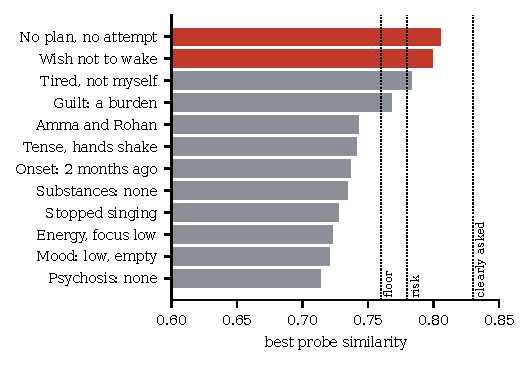
\includegraphics[width=\columnwidth]{fig_recall_example.pdf}
\caption{The twelve closest memories for ``Have you ever felt like you'd be better off not being around?'' (depression case). Red: risk memories.
Dotted lines: the cut-offs. The two risk memories pass the risk cut-off; the main complaint (0.783) passes the floor but is not a clear
winner, so it is not matched. Neither risk memory reaches 0.83, so neither counts as clearly asked.}
\label{fig:example}
\end{figure}

\section{The Benchmark}\label{sec:bench}

\begin{figure}[t]
\centering
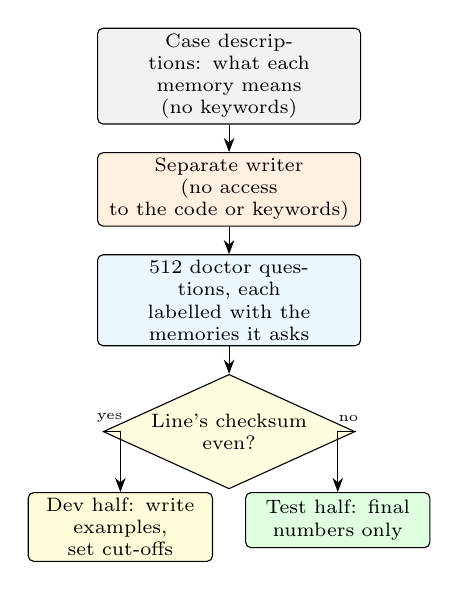
\begin{tikzpicture}[node distance=3.5mm]
\tikzset{b/.style={box=#1, text width=32mm}}
\node[b=gray!10] (a) {Case descriptions: what each\\memory means (no keywords)};
\node[b=orange!12, below=of a] (b) {Separate writer (no access\\to the code or keywords)};
\node[b=cyan!8, below=of b] (c) {512 doctor questions, each\\labelled with the memories it asks};
\node[decision, below=of c] (d) {Line's checksum\\even?};
\node[b=yellow!15, below left=4mm and -6mm of d, text width=22mm] (dev) {Dev half: write\\examples, set cut-offs};
\node[b=green!12, below right=4mm and -6mm of d, text width=22mm] (test) {Test half: final\\numbers only};
\draw[->] (a) -- (b); \draw[->] (b) -- (c); \draw[->] (c) -- (d);
\draw[->] (d) -| node[lab, above, pos=0.2]{yes} (dev); \draw[->] (d) -| node[lab, above, pos=0.2]{no} (test);
\end{tikzpicture}
\caption{How the blind benchmark was built and split.}
\label{fig:bench}
\end{figure}

Fig.~\ref{fig:bench} shows how the benchmark was made. A writer (an AI agent with no access to the code) was given only a description of each
case's memories: who the patient is, the kind of each memory, and what the patient knows. It was asked to write questions a real doctor might ask about each memory, following five rules. Write at least four lines per memory and twelve per risk memory. Mix textbook, gentle and indirect, clumsy, colloquial Indian English and euphemistic wording. Keep most lines free of the memory's own key words. Make every line understandable on its own. And add some ``none'' lines (greetings, small talk, pure empathy) that ask about nothing. It confirmed it read nothing else.

The result has 512 lines over four cases (176 depression, 154 alcohol withdrawal, 104 and 78 for two ward stations), including 38 ``none'' lines;
the writer marked 249 as hard. Table~\ref{tab:examples} shows examples. Labels are narrow: a matcher that also returns a neighbouring memory is not
penalised on recall, but those extras count as wrong matches. The split uses the CRC-32 checksum of each line: even lines form the \emph{dev} half,
which may be used for anything; odd lines form the \emph{test} half, used only for the numbers we report.

\textbf{Measures.} \emph{Recall} is the share of (question, expected memory) pairs where the memory is found. \emph{Risk recall} counts only risk
memories (suicidal thoughts, plans, means, withdrawal fits, anger at home), 77 pairs in the test half. \emph{Risk false hits} is the share of
questions that ask about no risk memory but are matched to one. We also report how many ``none'' lines match anything.

\begin{table}[t]
\caption{The benchmark by case}
\label{tab:benchstats}
\centering
\footnotesize
\begin{tabular}{@{}lcccc@{}}
\toprule
Case & Lines & ``None'' & Marked hard & Risk pairs\\
\midrule
Depression & 176 & 10 & 89 & 41\\
Alcohol withdrawal & 154 & 10 & 77 & 55\\
Ward: wants to go home & 104 & 9 & 52 & 41\\
Ward: refuses tablets & 78 & 9 & 31 & 15\\
\midrule
Total & 512 & 38 & 249 & 152\\
\bottomrule
\end{tabular}
\end{table}

Table~\ref{tab:benchstats} breaks the benchmark down by case. Almost half the lines are marked hard. The alcohol case has the most risk pairs,
because it has four risk memories (passive death wish, no plan, past withdrawal fit, anger at home).

\begin{table}[t]
\caption{Benchmark lines from the test half, and what each method found}
\label{tab:examples}
\centering
\scriptsize
\begin{tabularx}{\columnwidth}{@{}Ylc@{}}
\toprule
Doctor's line (expected memory) & Keywords & Hybrid\\
\midrule
Have you been saving up medicines or bought anything harmful? (no plan or means) & missed & found\\
Have you decided on a day or a method? (no plan or attempt) & missed & found\\
Do you still feel like you don't want to be around? (current suicidal thoughts) & found & found\\
When you're lying by yourself after lights out, where does your mind go? (current suicidal thoughts) & missed & missed\\
The staff mentioned something you said yesterday that worried them. Can we talk about it? (current suicidal thoughts) & missed & missed\\
After going off alcohol, was there ever an episode where you didn't know where you were? (withdrawal fit) & missed & missed\\
\bottomrule
\end{tabularx}
\end{table}

\section{Method}\label{sec:method}

\begin{figure}[t]
\centering
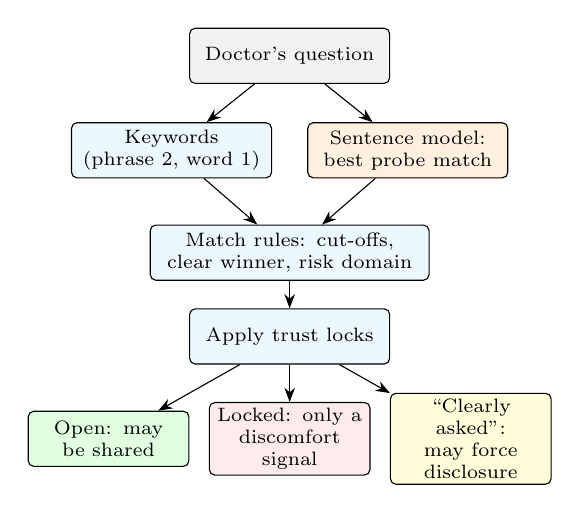
\begin{tikzpicture}[node distance=3.5mm and 4mm]
\tikzset{b/.style={box=#1, text width=24mm}}
\node[b=gray!10] (q) {Doctor's question};
\node[b=cyan!8] (lex) at ($(q)+(-15mm,-12mm)$) {Keywords\\(phrase 2, word 1)};
\node[b=orange!12] (emb) at ($(q)+(15mm,-12mm)$) {Sentence model:\\best probe match};
\node[b=cyan!8, text width=34mm] (rule) at ($(q)+(0,-25mm)$) {Match rules: cut-offs,\\clear winner, risk domain};
\node[b=cyan!8, below=of rule] (lock) {Apply trust locks};
\node[b=green!12, text width=19mm] (open) at ($(lock)+(-23mm,-13mm)$) {Open: may\\be shared};
\node[b=red!8, text width=19mm] (locked) at ($(lock)+(0,-13mm)$) {Locked: only a\\discomfort signal};
\node[b=yellow!15, text width=19mm] (strong) at ($(lock)+(23mm,-13mm)$) {``Clearly asked'':\\may force disclosure};
\draw[->] (q) -- (lex); \draw[->] (q) -- (emb); \draw[->] (lex) -- (rule); \draw[->] (emb) -- (rule); \draw[->] (rule) -- (lock);
\draw[->] (lock) -- (open); \draw[->] (lock) -- (locked); \draw[->] (lock) -- (strong);
\end{tikzpicture}
\caption{How a doctor's question is matched to the patient's memories. Matching ignores trust; the locks are applied afterwards.}
\label{fig:recall}
\end{figure}

Fig.~\ref{fig:recall} shows the method.

\textbf{Keyword layer.} Each memory has short keyword tags. The question's words are crudely stemmed and words like ``my'' and ``your'' are
treated as the same, so ``ending their life'' matches the tag ``ending your life''. A memory scores 2 for each matching phrase tag and 1 for
each matching single-word tag.

\textbf{Sentence-model layer.} We use bge-small-en-v1.5 \citep{xiao2023cpack}, a 33-million-parameter sentence model, run on the processor (not the
graphics chip). When a case loads, it turns every probe of every memory into a vector, once. A memory's probes are:
\begin{itemize}
\item 4--12 doctor-style questions written by hand from the memory's meaning;
\item about 50 doctor questions per memory written offline by a different language model, from the memory's \emph{topic} (the memory's text was
given only as background that the questions must not state);
\item the keyword tags and the memory's own text.
\end{itemize}

\textbf{Match rules.} A memory is matched if any of these hold: a keyword hit; similarity above 0.83 (0.78 for risk memories); or it is the best
match by at least 0.02 and above 0.76. If a question is clearly about risk, every risk memory within 0.06 of the best one is matched too,
because a locked risk match only makes the patient evasive. These values were chosen on the dev half (Table~\ref{tab:thresh}).

\begin{table}[t]
\caption{Cut-offs used (chosen on the dev half)}
\label{tab:thresh}
\centering
\footnotesize
\begin{tabular}{@{}lc@{}}
\toprule
Rule & Value\\
\midrule
Match on similarity alone & $\ge 0.83$\\
Match a risk memory & $\ge 0.78$\\
Best match, clear winner & $\ge 0.76$ and ahead by $\ge 0.02$\\
Risk domain: other risk memories & $\ge 0.66$ and within 0.06 of the best\\
``Clearly asked'' (may force disclosure) & keyword hit or $\ge 0.83$\\
\bottomrule
\end{tabular}
\end{table}

\textbf{Locks after matching.} Matching does not look at trust. The open/locked split is applied afterwards. So a cleverly reworded question about a
locked memory still produces only a discomfort signal, and locked text never enters the prompt.

\textbf{``Clearly asked''.} A stricter level marks what the doctor clearly asked about: a keyword hit or a similarity of at least 0.83. Only this
level may force the patient to disclose an unlocked risk memory, or count as a ``risk question'' for the patient's state. An ordinary match on a risk
memory never does.

\textbf{Hand-set heads (no training).} For five risk topics (suicidal thoughts, plans, means, harm to others, withdrawal) we wrote 10--17
example questions from clinical practice. Each topic's weight vector is simply the average of their vectors, scaled to length one:
\begin{equation}
w_k = \bar{e}_k / \lVert \bar{e}_k \rVert, \qquad \text{match if } w_k^\top e(u) \ge 0.76 .
\end{equation}
A question that passes the threshold is ``clearly asked'' for the memories tagged with that topic. There is no training step and no label made by a
model. The threshold was picked by hand from the dev curve (Table~\ref{tab:hand}).

\begin{table}[t]
\caption{Hand-set heads: choosing the threshold on the dev half}
\label{tab:hand}
\centering
\footnotesize
\begin{tabular}{@{}ccc@{}}
\toprule
Threshold & Dev risk recall & Dev risk false hits\\
\midrule
0.70 & 97.3\% & 38.9\%\\
0.72 & 96.0\% & 29.9\%\\
0.74 & 96.0\% & 24.8\%\\
\textbf{0.76} & \textbf{96.0\%} & \textbf{15.9\%}\\
0.78 & 93.3\% & 14.6\%\\
0.80 & 93.3\% & 12.7\%\\
\bottomrule
\end{tabular}
\end{table}

\section{Results}\label{sec:results}

\begin{table}[t]
\caption{Rank of the correct memory by probe similarity (dev half)}
\label{tab:ablation}
\centering
\footnotesize
\begin{tabular}{@{}llcc@{}}
\toprule
Sentence model & Probes & Top-1 & Top-3\\
\midrule
MiniLM-L6 \citep{wang2020minilm} & memory text & 0.534 & 0.777\\
MiniLM-L6 & text + label + tags & 0.580 & 0.857\\
MiniLM-L6 & hand-written questions & 0.706 & 0.866\\
MiniLM-L6 & questions + tags + text & 0.714 & 0.874\\
bge-small & hand-written questions & 0.744 & 0.916\\
bge-small & questions + tags + text & 0.739 & \textbf{0.933}\\
\bottomrule
\end{tabular}
\end{table}

\textbf{Questions match questions.} Comparing a question with example \emph{questions} works much better than comparing it with the memory's
\emph{statement} (Table~\ref{tab:ablation}). Hand-written probes raised the share of questions whose correct memory ranked first from 0.53 to 0.71
for MiniLM \citep{wang2020minilm,reimers2019sentencebert}, and bge-small \citep{xiao2023cpack} put the correct memory in the top three 93\% of the
time. The whole matching step took about 2\,ms per question.

\begin{table}[t]
\caption{Recall on the test half (never used for tuning)}
\label{tab:test}
\centering
\footnotesize
\begin{tabular}{@{}lcccc@{}}
\toprule
Method & All & Risk & Risk false hits & ``None'' hit\\
\midrule
Keywords only & 41.3\% & 35.1\% & 6.1\% & 22.7\%\\
Hybrid & 73.3\% & 72.7\% & 15.2\% & 22.7\%\\
Hybrid + hand-set heads & 74.9\% & 77.9\% & 21.2\% & 22.7\%\\
\bottomrule
\end{tabular}
\end{table}

\begin{figure}[t]
\centering
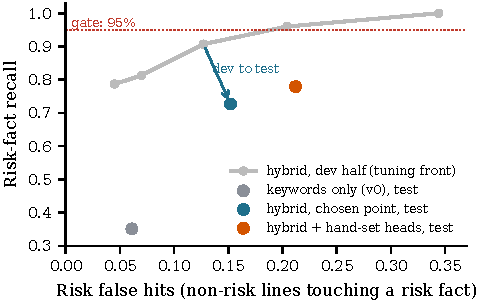
\includegraphics[width=\columnwidth]{fig_recall_front.pdf}
\caption{Risk recall against wrong risk matches. Grey: the trade-off on the dev half. Coloured: the test half. The chosen setting loses 18 points of
recall between dev and test.}
\label{fig:front}
\end{figure}

\begin{figure}[t]
\centering
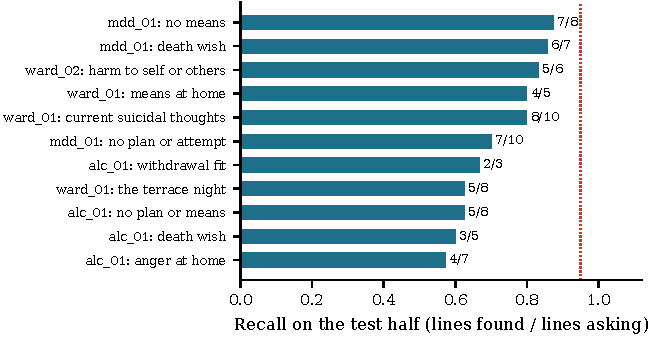
\includegraphics[width=\columnwidth]{fig_recall_byfact.pdf}
\caption{Recall per risk memory on the test half (red line: the 95\% target).}
\label{fig:byfact}
\end{figure}

\textbf{Test results.} Table~\ref{tab:test}: the hybrid method doubled risk recall compared with keywords, at about two and a half times the wrong
risk matches. Hand-set heads added 5.2 points of recall for 6.0 more points of wrong matches. The 95\% target was missed. Fig.~\ref{fig:byfact} breaks risk recall down by memory. Questions about the depression patient's death wish and means were found most often (6 of 7, and 7 of 8). Questions about anger at home, the passive death thought and plans in the alcohol case were found least (4 of 7, 3 of 5, and 5 of 8). Every wrong
match on a ``none'' line came from a keyword (``tell me'', ``morning'' in ``Good morning'', ``today''); the sentence model added no new wrong line.

\textbf{How sure are these numbers?} The test half holds 77 risk pairs. A bootstrap over those pairs gives a 95\% interval of 62.3\% to
81.8\% for the hybrid's risk recall. So the true figure could be ten points either side, but it is clearly far from 95\%.

\begin{table}[t]
\caption{Recall on the test half by case and by difficulty}
\label{tab:bycase}
\centering
\footnotesize
\begin{tabular}{@{}lcc@{}}
\toprule
& Keywords & Hybrid\\
\midrule
Depression & 36.6\% & 75.3\%\\
Alcohol withdrawal & 34.3\% & 61.2\%\\
Ward: wants to go home & 55.6\% & 77.8\%\\
Ward: refuses tablets & 45.5\% & 84.8\%\\
\midrule
Lines the writer marked easy (114 pairs) & 66.7\% & 92.1\%\\
Lines the writer marked hard (133 pairs) & 19.5\% & 57.1\%\\
\midrule
History memories (82 pairs) & 47.6\% & 74.4\%\\
Risk memories (77) & 35.1\% & 72.7\%\\
Symptom memories (60) & 45.0\% & 75.0\%\\
Triggers (16) & 50.0\% & 75.0\%\\
Formative memories (12) & 8.3\% & 58.3\%\\
\bottomrule
\end{tabular}
\end{table}

\textbf{By case and difficulty.} Table~\ref{tab:bycase}. The alcohol case is hardest: its memories (amount, morning drinking, a fit, anger) are
often asked about in slang and euphemism (``How many pegs would you have on a typical day?'', ``Have you ever got into trouble
with the police after a few pegs?''). The writer's own hard/easy marks predict
the result well: the hybrid finds 92\% of easy pairs and 57\% of hard ones; keywords find 67\% and 20\%. Keywords are close to useless on the
lines a real student is most likely to say when trying to be gentle. By kind of memory, the hybrid is even (73--75\%) except for formative
memories (guilt, shame, family history, readiness to change), which are often asked about indirectly (``How is your self-confidence?'',
``Tell me about your father's health.''). There are only 12 such pairs, so this figure is the least certain.

\textbf{Ranking is good; deciding is hard.} On the test half the correct memory had the highest similarity 73.3\% of the time, was in the top
three 92.3\% and in the top five 96.4\% (median rank 1). Yet only 73.3\% of pairs were matched. The sentence model nearly always puts the right
memory near the top; what fails is the decision of how far down the list to accept. Fig.~\ref{fig:sims} shows why. Correct pairs have a median
similarity of 0.82, but their spread overlaps the best \emph{risk} similarity of non-risk questions: 11.2\% of non-risk questions score at least
0.78 against some risk memory. No single cut-off separates the two.

\begin{figure}[t]
\centering
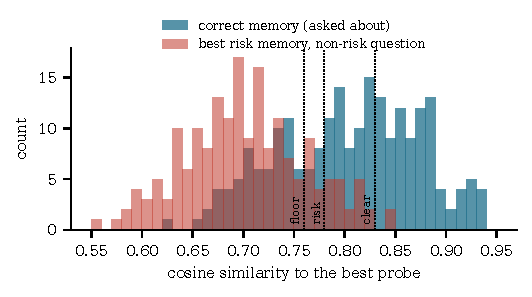
\includegraphics[width=\columnwidth]{fig_recall_sims.pdf}
\caption{Test half. Blue: similarity of each question to the memory it asks about. Red: for questions that ask about no risk memory, the
highest similarity to any risk memory. Dotted lines: the cut-offs. The two overlap, so a cut-off trades recall for wrong matches.}
\label{fig:sims}
\end{figure}

\begin{table}[t]
\caption{Which probes matter (test half, reported only)}
\label{tab:probes}
\centering
\footnotesize
\begin{tabular}{@{}lcc@{}}
\toprule
Probes used & All & Risk\\
\midrule
Hand-written + generated + tags + text (shipped) & 73.3\% & 72.7\%\\
Hand-written + tags + text & 66.8\% & 63.6\%\\
Generated + tags + text & 62.3\% & 64.9\%\\
Tags + text only & 44.9\% & 37.7\%\\
\bottomrule
\end{tabular}
\end{table}

\textbf{Which probes matter.} Table~\ref{tab:probes} removes each source of probes in turn, keeping the cut-offs fixed. Example questions of
either kind add about 20--27 points over tags and memory text alone, and the two kinds add to each other: hand-written and generated probes
together beat either alone by 6--9 points. So the generated probes help overall, even though some of them are off-topic (below).

\textbf{Kinds of miss.} Of the 21 missed risk pairs, 8 matched nothing at all, 8 matched only a non-risk memory, and 5 matched a
different risk memory. The last group does little harm in practice: a locked risk match still makes the patient evasive.

\textbf{Speed.} Matching one question, including the keyword pass, the sentence model and the rules, took 3.0\,ms at the median and 3.7\,ms at the
90th percentile on the laptop's processor. The first call of a session takes about 5\,s while the model loads, so the service loads it at start-up.

\textbf{Why questions were missed.} Table~\ref{tab:misses} groups the 21 missed risk questions in the test half by type, with real examples.
Most are euphemisms without any risk words, questions about a situation rather than the thought itself, or open questions that leave the topic to
the patient. A real clinician would recognise all of them as risk questions.

\begin{table}[t]
\caption{Missed risk questions on the test half, by type}
\label{tab:misses}
\centering
\scriptsize
\begin{tabularx}{\columnwidth}{@{}lY@{}}
\toprule
Type & Real example (expected memory)\\
\midrule
Euphemism & ``Do you ever feel like you just want it all to stop?'' (death wish)\\
Situation, not thought & ``If these feelings got worse tonight, do you think you would do anything about them?'' (no plan)\\
Open question & ``In your lowest moment recently, what was going through your mind?'' (passive death thought)\\
Other people's angle & ``Have you ever thought your family would manage better if you weren't there?'' (passive death thought)\\
Matched a nearby topic & ``Have you googled anything about overdoses?'' $\to$ matched substance use instead (no means)\\
Indirect action & ``Have you ever swallowed something or cut yourself in a bad moment?'' (no plan or means)\\
Physical wording & ``Do things ever get physical at home?'' $\to$ matched consequences (anger at home)\\
\bottomrule
\end{tabularx}
\end{table}

\textbf{The gap between tuning and test.} The chosen setting scored 90.7\% risk recall on the dev half and 72.7\% on the test half
(Fig.~\ref{fig:front}). An earlier setting, tuned after we had also written probes inspired by dev-half misses, scored 98.7\% on dev and 72.7\% on
test. The dev half was used twice (to write probes and to set five cut-offs) on only about 75 risk pairs, which is enough to fit the dev half
closely without improving on new questions.

\textbf{Some generated probes were off-topic.} We checked the questions the other language model wrote for risk memories: by a simple word list,
46\% (245 of 533) contain no risk-related word at all. Some of those are fair indirect questions, such as ``Have you felt that life has lost its meaning?''. But some are plainly off-topic. For example, ``Before we continue, could you tell me a bit about how you have been sleeping lately?'' was listed as a probe for the death wish. This explains why sleep questions matched suicide memories, and shows that generated probes need a quality filter.

\textbf{Tuning for recall alone is unsafe.} An automatic re-tune that tried only to maximise dev risk recall reached 100\% on the dev half, but
its settings matched 36.9\% of non-risk dev questions to a risk memory (37.6\% on the test half, Table~\ref{tab:sweep}). In held-out conversations, the patient then treated ``How have you been sleeping, and how is your appetite?'' as a suicide question, and answered about sleep but not appetite. In 3 of 98 turns it mentioned the death wish without being asked. Separating ``matched''
from ``clearly asked'' and capping wrong risk matches fixed it.

\begin{table}[t]
\caption{Moving the risk cut-off (other settings as shipped)}
\label{tab:sweep}
\centering
\footnotesize
\begin{tabular}{@{}lcccc@{}}
\toprule
& \multicolumn{2}{c}{Dev half} & \multicolumn{2}{c}{Test half}\\
Risk cut-off & Recall & False hits & Recall & False hits\\
\midrule
0.72 & 100\% & 34.4\% & 89.6\% & 34.5\%\\
0.74 & 98.7\% & 23.6\% & 83.1\% & 25.5\%\\
0.76 & 93.3\% & 17.8\% & 76.6\% & 19.4\%\\
\textbf{0.78 (shipped)} & \textbf{90.7\%} & \textbf{12.7\%} & \textbf{72.7\%} & \textbf{15.2\%}\\
0.80 & 81.3\% & 8.9\% & 70.1\% & 12.7\%\\
0.82 & 81.3\% & 5.1\% & 66.2\% & 9.7\%\\
0.84 & 78.7\% & 4.5\% & 66.2\% & 8.5\%\\
\midrule
Recall-only tune & 100\% & 36.9\% & 84.4\% & 37.6\%\\
\bottomrule
\end{tabular}
\end{table}

\textbf{The trade-off, measured.} Table~\ref{tab:sweep} moves only the risk cut-off and reports both halves (the test columns were computed
after the cut-off was fixed, for this paper only). Every step down buys a few points of recall for several points of wrong matches. To reach
the 95\% target on new questions, the cut-off would have to go below 0.72, where more than a third of ordinary questions already look like risk
questions. This is the clearest evidence that cut-offs on this sentence model cannot meet the target, and that better training data, not a
better cut-off, is needed.

\subsection{Learning the match instead of setting it}
We also tried to learn the reading of a doctor's line from data, using the three kinds of simulated doctor that a real teaching programme meets.

\textbf{Data.} A language model wrote doctor lines for every topic the debrief scores and every move the rubric reads. It wrote them in the voice of three kinds of doctor. The first is an experienced psychiatrist: precise, calm and normalising. The second is a nervous medical student: clumsy, blunt, sometimes asking two questions at once. The third is a tester trying to break the simulator: rude, sarcastic and repetitive, but still on topic. We added 369 doctor lines from the developer's
own test sessions and removed anything close to a held-out line. A judge model from another family (Qwen3.5-9B) then labelled each line with
the topics and moves it contains.

\begin{table}[t]
\caption{Training data for the learned classifiers}
\label{tab:train}
\centering
\footnotesize
\begin{tabular}{@{}lcc@{}}
\toprule
Source & Lines & Judge agrees with intended topic\\
\midrule
Simulated psychiatrist & 1,113 & 56.1\%\\
Simulated student & 1,089 & 55.5\%\\
Simulated tester & 1,099 & 38.8\%\\
Developer's sessions & 369 & --\\
\midrule
Total & 3,670 & 50.1\% (generated lines)\\
\bottomrule
\end{tabular}
\end{table}

\textbf{The labels were the problem.} Table~\ref{tab:train}: the judge agreed with the topic each generated line was written for only half the
time, and for the tester's lines only 38.8\%. Some disagreements are the generator's fault (a ``risk'' line that really asks about sleep, as with
the probes above), some the judge's (a rude line about medicine labelled only as abuse). Either way, half the labels a classifier would learn from
are doubtful.

\textbf{Model.} One logistic-regression head per label on the frozen sentence vector that recall already computes, so it costs well under a
millisecond per turn. 53 of the 57 labels had at least 8 examples; thresholds were set by cross-validation.

\begin{table}[t]
\caption{Learned classifier against the current methods (381 held-out lines, judge-labelled)}
\label{tab:clf}
\centering
\footnotesize
\begin{tabular}{@{}llcc@{}}
\toprule
Task & Method & Micro-F1 & Macro-F1\\
\midrule
Manner (rubric moves) & Word patterns (live) & 0.198 & 0.347\\
& Learned classifier & 0.322 & 0.334\\
\midrule
Topic (debrief intents) & Language-model tagger (live) & 0.692 & 0.672\\
& Learned classifier & 0.657 & 0.577\\
\bottomrule
\end{tabular}
\end{table}

\textbf{Results.} Table~\ref{tab:clf}. The learned classifier read the \emph{manner} of a line better than the word patterns overall (micro-F1 0.32 against 0.20), but not per label (macro-F1 about equal). It read the \emph{topic} worse than the language-model tagger. A patient
version using it scored lower in held-out conversations, so it was not shipped. A separate risk-topic detector trained only on the intended topics
found 87\% of risk questions in cross-validation, but only 35\% of what it flagged really was a risk question. The held-out labels came from the
same judge and have not been checked by hand, so these F1 values are themselves uncertain. The lesson is the same as for recall: with labels this
noisy, a learned model cannot beat simple rules, and a few hundred hand-checked labels are worth more than thousands of generated ones.

\section{Discussion}
\textbf{Practical lessons for builders.}
\begin{enumerate}
\item Write the test questions \emph{blind}, from what the memory means, never from the matching rules.
\item Keep a test half that is never touched; report it, not the tuning half.
\item Always report wrong risk matches next to risk recall.
\item Use a stricter ``clearly asked'' level for anything with consequences, such as forcing a disclosure.
\item Compare questions with example questions, not with statements.
\item Check generated examples for topic before using them.
\end{enumerate}
Hand-set heads are attractive when labels are few or noisy: they take minutes, anyone can read them, and they keep memory text out of any trained
weights. Here they helped only a little. The next step is a small, hand-checked set of labels and a fine-tuned sentence model; the code exists but
was not run for this paper.

\textbf{Limitations.} One writer produced the benchmark, with narrow labels. About 75 risk pairs per half means each recall figure is uncertain by
several points. There are four cases, all in one variety of English. The judge-labelled set used for the trained classifiers was not checked by
hand. Speed was measured on one laptop. The session logs used for training were the developers' own tests; the pipeline now only accepts logs from
sessions where consent was recorded.

\textbf{Threats to validity.} The benchmark writer was an AI agent, so its phrasing may be more regular than a nervous student's. Labels are
narrow and were written with the questions, so a reasonable extra match can count as wrong. The dev and test halves come from the same writer,
so the test half measures new wording, not a new writer; a second, human-written set would be stronger. Cut-offs were chosen by hand from a
curve, which is less over-fitted than automatic tuning but still used the dev half.

\section{Conclusion}
Combining keywords with a small sentence model, and applying trust locks after matching, doubles the recall of suicide-related questions asked in
new words, at little cost in time. It still falls well short of what a safety gate needs, and a tuning half reused for writing examples makes it
look nearly twenty points better than it is.

\section*{Software and data release}
The benchmark, its split, the matching code, the probes and the cut-off file will be released under an open licence with the final
version.

\section*{Use of AI tools}
The text of this article, its figures, tables and analysis scripts, and the \LaTeX{} source were
drafted with an AI assistant (Claude, Anthropic, used through Claude Code), working from the project's code, experiment logs and result
files under the authors' direction. The same assistant helped write the software described here, ran the analyses, and checked the
citations against their sources. Within the study itself, AI models were also used as research tools, as described in Sections~\ref{sec:bench} and~\ref{sec:method}: an AI agent wrote the blind benchmark, a language model wrote the generated probes, and a judge model labelled the classifier data. The authors take full responsibility for the content of this article.

\bibliography{../../shared/refs}
\bibliographystyle{acl_natbib}
\appendix
\section{Instructions given to the benchmark writer}
The writer received, for each case: the patient's name, age and situation; for each memory its id, its kind (complaint, symptom, history, risk,
social, belief) and a one-line description of what the patient knows; and these rules: write lines a real doctor might say to this patient;
at least 4 per memory and 12 per risk memory; mix textbook, gentle and indirect, clumsy and leading, colloquial Indian English, and euphemistic
phrasings; most lines should avoid the memory's obvious key words; each line must make sense on its own; label each line with every memory it
asks about, and nothing more; include greetings, small talk and empathy-only lines that ask about nothing; mark hard lines. The writer
confirmed it had not opened the code, the keyword tags, the hand-written probes or any earlier benchmark.

\section{Hand-set heads: example questions}
Each head is the normalised average of its example questions' vectors. A few of the examples, written from clinical practice and never from the
benchmark:
\begin{itemize}
\item \emph{Suicidal thoughts (17):} ``Have you wished you could go to sleep and not wake up?'', ``Do you sometimes feel everyone would be better
off without you?'', ``When it gets very heavy, do thoughts of death come to you?''
\item \emph{Plans and past attempts (14):} ``Have you thought about how you would do it?'', ``Have you done anything to prepare, like writing a
note?'', ``Can you keep yourself safe if you go home today?''
\item \emph{Means (12):} ``Have you been saving up medicines?'', ``Can you get onto a roof or somewhere high easily?'', ``Is your home safe for
you right now?''
\item \emph{Harm to others:} ``Has anyone at home been afraid of you?'', ``Have arguments ever got physical?''
\end{itemize}

\section{Reproducing the results}
\texttt{tools/recall\_bench.py --split test} prints recall and wrong-match rates for the shipped settings; \texttt{--lexical} gives the keyword
baseline and \texttt{--hand} adds the hand-set heads. \texttt{papers/analysis/analyses.py --recall} and \texttt{recall\_extra.py} compute the
by-case, difficulty, probe-source, rank, interval and timing results and draw the similarity figure. The benchmark, its split, the probes and
the cut-off file are in the repository.
\end{document}
